\part{Solution} \label{part:solution}

\chapter{IoT Monitoring Tool}

This chapter will be the occasion to detail the architecture of our solution. We will explain the technologies employed to achieve our goal, a monitoring software for Internet of Things networks. It is also in this chapter that we will justify the choices we made during the development of it.

\section{Architecture}

The architecture of our solution is composed of two parts as can be seen on Fig.\ref{fig:design}. The first part is about how the data is collected and sent. The second part consists of how the data is received and treated after reception. In the remaining of the section, strong assumptions are made that the reader is familiar with Netflow, particularly IPFIX, also referred as Netflow v10, and also its implementation for WSN which is called TinyIPFIX. If not, explanations about those particular technologies can be found in Chap \ref{chap:monitoring_tools}. \\

\begin{figure}
	\centering
	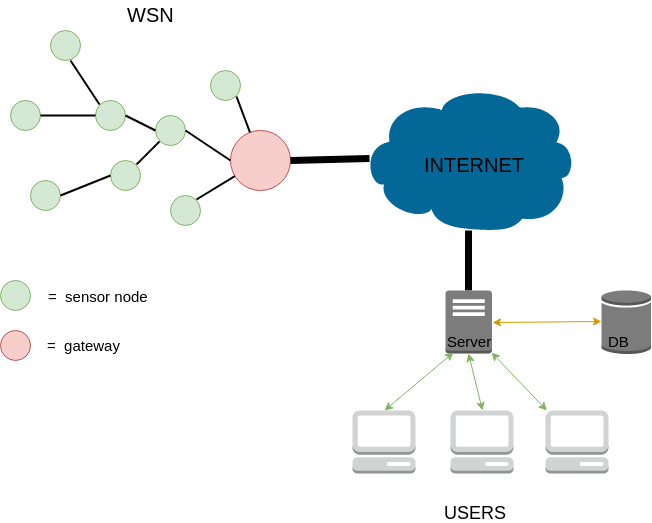
\includegraphics[width=0.8\textwidth]{res/design.png}
	\caption{Global architecture of the solution}
	\label{fig:design}
\end{figure}

The data exportation is done in a Netflow fashion. The nodes occupy the role of exporters. Each node maintains a flow table where they register the flows that occurred during an interval of time. In our case, a flow is characterized by the 4-uple: source node id, destination node id, number packets and number octets. After a certain amount of time, each node will construct a TinyIPFIX message based on the content of its flow table. Those messages are sent to the gateway node. The gateway node will then reformat the TinyIPFIX messages received into compliant IPFIX messages to a specific address, which will be in our case the address of a server.\\

The server that receives the IPFIX messages from the IoT network plays two roles. One role is straightforward, it plays the role of collector. Each message is collected by the server and logged in a database for further processing and analyzing. The other role is of a web server. Multiple users can know the network status by having access to web pages served by the server.

\section{Technologies}

The monitoring tool developed for this thesis is a \textit{web-based} solution. We've chosen to write the monitoring tool with \textbf{Node.js} \cite{website:nodejs} which is a server-side solution for Javascript. In that sense, it offers modules or API to effectively develop HTTP/HTTPS server, meaning web server. To speed up our development, we used the \textit{Express framework} \cite{website:express} on top of Node.js. Express simplify the routing of requests to views. A view can be seen as an web page. \\

The reasons we've chosen to write our monitoring tool as a web-server is the portability of such a solution. All OSs dispose of a web browser. For the user, it simplifies the utilization of the tool by simply accessing the web site via its preferred browser. The user does not have the trouble to download and install our software as with common desktop applications. Also, the user can freely access the tool from different locations and computers. He is not limited to devices where the software is installed on. \\

Another factor in favor of a web solution is the ease with which multiple users can access the software in the same time. Most of the monitoring tools presented are desktop applications. They take the role of collectors and store the logs in a local database. This implies that the nodes transfer their data directly to the device having the monitoring tool on. However, a considerable drawback of such design is when multiple administrators exist for a same IoT network. Multiple users are bound to one device to monitor the network. One approach would be to retransmit the data sent by the nodes to each devices containing the monitoring tool in question, but it does not scale well. The web solution is not limited by that. By having a centralized server playing the role of collector but also of web server, different users can efficiently monitor the network on their own device by simply requesting the web server. \\

One of the reasons for developing the software with Node.js and not other particular frameworks like Django or Ruby on Rails is due to the features that it offers via notably the Javascript language. First, it is event-driven and asynchronous by nature which is what we desire for our product. One such event to react to is when the collector receives an IPFIX message. Other events are when the status of a node changes as you will see later on. Programming by events proved powerful in our case. Secondly, the huge support on the Javascript language and its popularity which makes it a good choice for the adoption of the tool. Additionally, the huge documentations and modules helped us develop the tool faster and better. Thirdly but nonetheless, Javascript is tightly coupled to JSON (Javascript Object Notation) \cite{website:json} which is a data-interchange format. Objects in Javascript can be easily formated to JSON formated and exchanged via Internet. This allow to make dynamic website. Finally, we limit the language used during the process of production of the software mainly to Javascript for backend and HTML, CSS and Javascript for frontend where other frameworks would impose to master one or two more languages.\\

HTML, CSS and Javascript which are the core means to present web pages proved to be useful but also easy to produce ways of visualizing the data. Javascript presents a lot of library to display graphs, charts and other type of figures. One such popular library is D3.js \cite{website:d3}. It also enables a website to be dynamic. Popular libraries like Bootstrap helped in making web page quicker and saved us the trouble to modify CSS files.\\

For the database, \textbf{PostgreSQL} \cite{website:postgresql} was used. It is an open-source relational database system. With more than 15 years of development, it does not have to prove anything anymore in term of reliability. It is SQL compliant. It recently added the support of JSON as field which enabled us to save IPFIX messages as JSON objects and not simply binary data.

\section{The monitoring tool}

This section will detail the different modules that compose our application plus the features that are offered by our application.

\subsection{Modules}

The application is comprised of four different modules :
\begin{itemize}
	\item Collector
	\item Log
	\item Nodes Status
	\item Web \\
\end{itemize}

The \textit{Collector} consists of a UDP server that listens to incoming IPFIX messages. Upon reception of a message, the Collector parses the binary data into an IPFIX object representing the original message. The object created is what will be used for the application to work with. It offers methods to read records contained in the original IPFIX object. The Collector emits an event each time it creates an object from a received message. Modules can then listen and react to this particular event and treat the newly created object. \\

The \textit{Log} module offers logging capabilities of IPFIX message. It also gives the possibility to query it. The storing is done in a PostgreSQL database. However, users can freely switch to its SQL prefered database as long as it also offers the possibilty to create a JSON field. To log an IPFIX message, it listens to the Collector's event mentioned before. It then stores in the database the JSON representation of the object. The module proposes methods to query the database such as having the different flows between two nodes as example. As to enhance the reactivity of our application, other tables are created apart from the ones that contained the IPFIX objects. One such table is the different flows.\\

To keep track of the status of the nodes, we deemed necessary to create a \textit{Nodes Status} module. This particular module also listens to the Collector's event for incoming IPFIX object. It will then update the status of the nodes according to the content of the object. The status of a node comprises its parent, its battery, its number of bytes sent, number of packets sent and the last packet sent, to name a few. The Nodes Status module offers the current state of the different nodes contained in the IoT network. To retrieve past values, it is necessary to pass via the Log module. \\

The final module is the \textit{Web} one. This module is essentially an HTTP server. Users interact with our tool mainly via this module. It permits users to visualize the status of their network via their browser by launching HTTP requests to which the server will reply by delivering the requested content. This module is an intermediate between the users and the Nodes Status module but also between the users and Log module. The reason for that is, to deliver content to the users, this module needs to gather data which is contained by the two aforementioned modules. This module can be seen as the frontend of our application whereas the others can be viewed as composing the backend of our solution.\\

The reasons behind using multiple modules is to achieve one of the requirement we imposed on ourselves, the \textit{modularity} of our program. We stated that a user should easily extend our software to add new features. By separating our applications into four different modules, we achieved this requirement. Each module offers different functionalities and abstractions. The Collector is responsible of collecting the IPFIX messages, the Log module to log those messages and provide means to query the logs, the Nodes Status keep track of the status of the IoT network and finally the Web module permits users to interact and visualize the data. Users wanted to add another web page will mostly only look into the Web module by adding another route to which the server will respond by replying by an HTML page. \\

The Fig.\ref{fig:modules} depicts the different modules presented and their interactions. As shown in the figure, the modules occupy different layers. The first layer is occupied by the Collector. The second one is occupied by the Nodes Status and Log modules. And finally the third one is composed solely of the Web module.

\begin{figure}
	\centering
	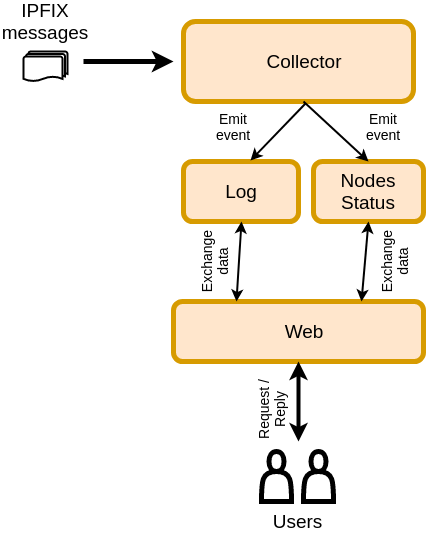
\includegraphics[width=0.5\textwidth]{res/modules.png}
	\caption{Modules interactions}
	\label{fig:modules}
\end{figure}

\subsection{Features}

The features offered by our monitoring applications are what we considered to be the basic ones.

\todo[inline]{Add screenshots of the sotware + detail more + add features}
\begin{description}
	\item[Topology Map] Display the logical topology of the WSN. The topology represents the RPL routing, meaning the topology is actually acyclic and represents a tree. A link represents a relation of parent-child between two nodes. The root is the gateway node, and is colored differently to distinguish it from leaf nodes, which do not have children. Each node composing the topology is associated with its unique respective ID. Moreover, those nodes are uniquely clickable, one at a time, to get further information about their node values.
	\item[Node values] Offers the possibility to see more in depth the values sent by a particular node. With these features, an administrator has the possibility to see how the different values have evolved in time. It also gives meaningful statistics as the average number of bytes sent by interval of time, how often it is addressed and so on.
	\item[Network statistics] Gives statistics which are general to the whole network. This comprises the amount of traffic generated by the network. But also gives meaningful insight about the node having the less battery or the node sending the most data. This gives a broad view to the administrator.
\end{description}

\chapter{Alternatives}

\section{Nfsen, A Graphical Web Tool}
\begin{figure}[!h]
	\centering
	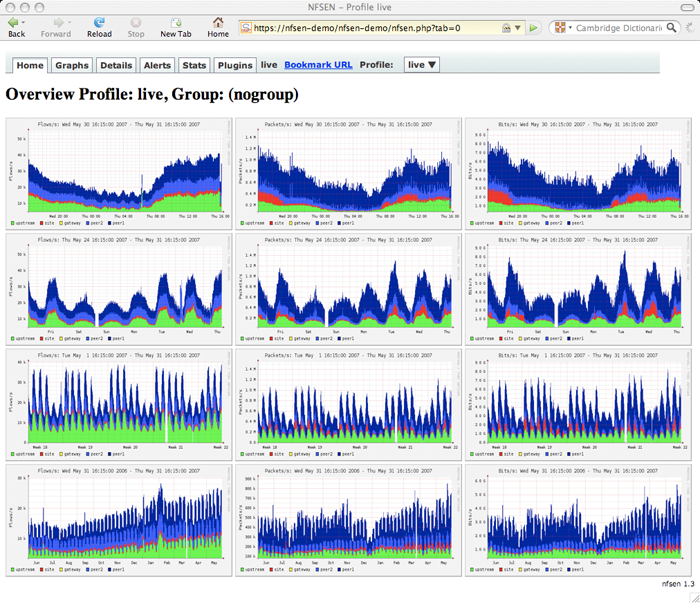
\includegraphics[width=0.8\textwidth]{res/nfsen.png}
	\caption{The Nfsen interface (source : http://nfdump.sourceforge.net/)}
	\label{fig:nfdump}
\end{figure}

The subject of our master thesis having been proposed by Professor Sadre last year and being about monitoring flows in IoT networks, the first tool that was presenting itself to us was Nfsen. Per its official website, \textit{Nfsen is a graphical web based front end for the nfdump netflow tools}. The Nfsen tool uses various graphes and charts to display the traffic of data varying with a specified time span or time interval. It works with the processing capabilities of Nfdump, a data processing tool using Netflow flows that have been retrieved from a network. Specifically, the Nfsen interface also allows to create plugins to have more ways of displaying data information. At first, it was proposed in the description of the subject of the thesis to use Nfsen along with Nfdump, particularly creating an Nfsen addon to show further information along with what Nfsen already is displaying in terms of graphical content. By plugin, one graphical content that Nfsen is lacking is the current topology of the monitored network, which can be added by making a plugin which extends the graphical tool.\\

In this section, we will explain all the underlying layers of Nfsen, from data exchanged in the monitored network to the graphical web page. We will also discuss our thought process about using Nfsen and the reasons why we have not used it in the end.\\

The first step towards monitoring is data collecting. As we explained in Chapter 3, Netflow is used for collecting flows we are interested in, according to some specific attributes such as the source and destination addresses. Once the flow are captured, they are stored and waiting to be processed. \\

(source : http://nfdump.sourceforge.net/, https://www.first.org/conference/2006/papers/haag-peter-papers.pdf)
In reality, when the structure of the Netflow data is defined, the flows are actually captured by \textit{nfcapd}, a \textit{netflow capture deamon}. With nfcapd, the flows are read from the network and the collected data is stored into files, data being split in files according to time slices. Each five minutes, nfcapd outputs a new file where data is stored, named with the current timestamp. One nfcapd process is used for each existing netflow stream that we want to capture.\\

As seen in the next figure, the next important component is \textit{nfdump}. Nfdump is a command line based tool that provides further data processing. Basically, it reads the data that was previously captured and stored by nfcapd. With Nfdump, data is aggregated and it provides further statistics about the traffic. Nfdump can either analyze the data coming from a single file, or from several of them by concatenating them before analyzing. One strength of nfdump is that it can filter out the attributes in the data that are not needed during the processing. Afterwards, the data is output either as a text file or binary data, thus being ready for further analysis. Nfdump aggregates and then creates statistics about the flows information stored, such as traffic volume sent during a timelapse. Nfdump thus acts as the backend of Nfsen.\\

\begin{figure}[!h]
	\centering
	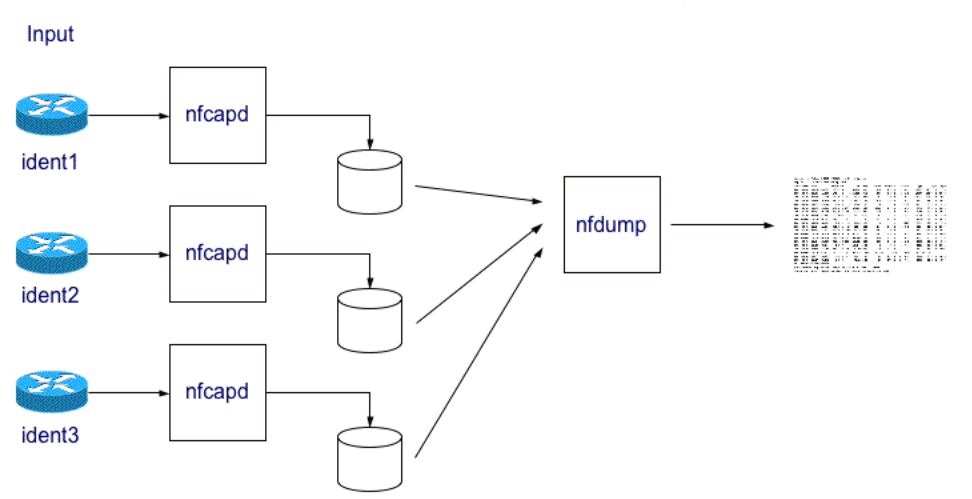
\includegraphics[width=0.8\textwidth]{res/nfdump.png}
	\caption{The Nfdump Structure (source : http://nfdump.sourceforge.net/-)}
	\label{fig:nfdump}
\end{figure}

Once the data is processed, it is displayed by Nfsen with the help of graphs. Nfsen displays the collected netflow data, either in flows, packets, or bytes. As you can see in figure \ref{fig:nfsen}, it can display various types of data, for example data sent through different protocols such as UDP, TCP, etc. It also uses time spans to select which data traffic is to be displayed (being the same time spans where nfdump did all the processing).\\

As stated earlier, Nfsen can also be extended, by creating plugins. There exist two kinds of plugins. There are the backend plugins that are written in Perl, that are created to add more functions and functionalities such as alerting conditions and data processing. On the other hand, frontend plugins are written in PHP and used to create new display fashions that the original Nfsen application would lack. In our case, we wanted to display the topology of the network under analysis, which Nfsen is not showing in its original state. Note that each backend plugin should be associated with its respective frontend plugin.

\section{Nfsen \& Nfdump, not best suited?}

In section 5.1, we talked about Nfsen and how it is possible to create plugins to have further monitoring capabilities. As stated, the first description of the thesis was to create an \textit{Nfsen plugin} to visualize an IoT network in an Ad Hoc manner, with devices having Netflow activated.\\ 

At the beginning of this school year, once we started working on our thesis, we dug into Nfsen and its functionalities, trying to get familiar with it. First of all, setting up the Nfsen tool showed itself to be very tedious and challenging, as many installation tutorials did not work for all computers and OSs, and had different instructions.\\

The main reason why Nfsen is useful is that it easily and immediately treats the netflow information retrieved by nfcapd and nfdump, with little to no addition and/or modification needed. However, as we had decided to modify the netflow structure to visualize IoT networks according to our needs, we also had to modify nfdump. Namely, two fields that the original netflow structure does not monitor, and hence are not standardized fields, are the battery level of devices and the parent of each mote in the IoT networks. Digging into nfdump seems to require quite some time and some knowledge of the Perl language. Entering the last year of our master thesis, we also had never used nor learned the PHP and perl languages in contrary to Javascript with the Node.js framework. \\

Thinking of using the Node.js framework seemed reasonably more practical in our case in terms of time allocation, since we required to modify the netflow information retrieved from networks. With further discussion, we decided to write a Javascript program that played the role of Nfdump to efficiently parse and store the netflow information captured. Similarly, instead of using nfsen as the graphical interface, we programmed a web tool with Node.js to be able to visualize information in which we are interested in. Of course, our graphical interface is less complete than nfsen's, but it contains a topology showcase that nfsen does not, that we have programmed using the D3.js framework as explained earlier.\\

In the end, Nfsen used with Nfdump present a lot of advantages, as most of the work is already present in its core, only a few things have to be added, i.e. the topology here. It contains a lot of graphical information on how much traffic passes through the network, with many filters such as graphs split according to which protocols send the information. But for the reasons we have cited above, we have decided not to use it and opted for a solution using Node.js. 

\todo[inline]{explications techniques en plus ?}

